%\begin{figure*}[tb]
%  \centering
%  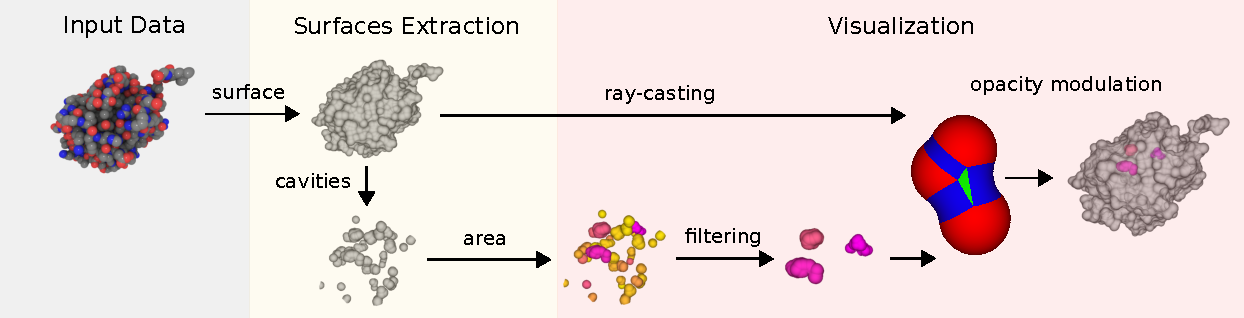
\includegraphics[width=\textwidth]{image/overview_final.pdf}
%  \caption{Illustration of the visualization pipeline. The input data (Sec.~\ref{ch:overview}) contains snapshots of MD trajectories which are processed to construct the molecular surface and cavities (Sec.~\ref{ch:feature}). Then, the surface areas of cavities are estimated (Sec.~\ref{sec:area}), which are used as the color codes, ranging from yellow (smallest) to magenta (largest). These areas serve for filtering out of too small cavities. Finally, the surface elements are ray-cast (Sec.~\ref{sec:spherical-patches}) to compose the surface fragments used in the final stage to visualize the surfaces transparently via a user-defined opacity modulation (Sec.~\ref{sec:opacity}).}
%	\label{fig:overview}
%\end{figure*}

The computation of SES is not a trivial task and requires substantial computation and algorithmic capabilities. 
Therefore, a technique that could provide the users with an instant computation and interactive and meaningful visualization of cavities in the context of molecular surfaces would be highly beneficial.

The input data comes in a form of MD trajectories describing the motion of individual atoms. 
Each trajectory snapshot includes a set of atoms, described by their positions and radii. 
Our rendering pipeline consists of several steps that are performed on a per-frame basis. 
For better explanation, we split the computations into two groups. 
The first group deals with data processing that involves the computation of the surface patches and inner voids, i.e., cavities.
The second group of computations focuses on visualization of the generated patches. 
This group includes the estimation of area of cavities, ray-casting the SES patches, and opacity calculation; performed before the final stage represented by the image formation. 
More specifically, our pipeline consists of the following steps (Fig.~\ref{fig:overview}):
	\begin{enumerate}
	  \item We employ the contour-buildup algorithm to construct the molecular surface. Additionally, we enhance the computation to enable i) transparent rendering of the surface and ii) extraction of cavities (Sec.~\ref{sec:ecb}).
		\item For cavity extraction, we utilize the so-called \textit{surface graph} (Sec.~\ref{sec:graph}), which allows us to detect the isolated surface components.
		\item We estimate the area of the extracted cavities to enable color coding by their size and to decrease the potential clutter by hiding small cavities.
		\item Surface elements are visualized using ray-casting (Sec.~\ref{sec:vis}). We perform transparent surface rendering by means of the A-buffer and the opacity modulation. The modulation is based on an estimate of the molecular thickness per each surface fragment on a given ray and a set of user-defined parameters.
	\end{enumerate}
	
In the following we focus on a detailed description of these individual steps.